\chapter{MySQL DDL parser}
Na základe dôvodov popisovaných v poslednej kapitole, som sa na implementáciu DDL parseru pre MySQL rozhodol použiť nástroj ANTLR verzie 4. Tento nástroj je aktuálne vo svete asi najpoužívanejší a prináša veľké množstvo výhod, ktoré uľahčujú implementáciu aj následne ladenie parsovacích programov.

\section{Základy ANTLR v4}

Štvrtá verzia ANTLR má niektoré dôležité nové možnosti, ktoré znižujú učiacu sa krivku a umožnuje vytvárať gramatiky a jazykové aplikáciie oveľa jednoduhšie. Najdôležitejšou výhodou je, že ANTLR v4 akceptuje každú gramatiku, ktorú mu poskytnete (s výnimkou týkajúcou sa nepriamej ľavej rekurzie). ANTLR prekladá vašu gramatiku do spustiteľného, ľudsky čitateľného analytického kódu, do ktorého keď zadáte platný vstupný reťazec, parser vždy rozpozná vstup správne, nezávisle na komplikovanosti gramtiky.

V rámci tejto sekcie sú popísané základné informácie potrebné na pochopenie toho, ako s ANTLR pracovať. Na získanie podrobnejších alebo viac detailných informácií doporučujem knihu \textit{The Definitive ANTLR4 reference}\cite{definitiveANTLR} napísanú autorom ANTLR nástroja.

\subsection{Nastavenie ANTLR}
ANTLR sa skladá z dvoch častí: Nástroja na generovanie lexeru a parseru z gramatiky a knižnice potrebnej na beh parseru.

Nástroj na generovanie je rovnaký, nezávisle na výstupnom jazyku generovaného lexeru a parseru, a pre samotný beh parseru nie je potrebný. Využijú ho užívatelia, ktorí vytvárajú, alebo upravujú gramatiku. Je to vlastne program napísaný v programovacom jazyku Java, a preto je nutné na prácu s ním mať nainštalovanú aspoň Javu 1.7. Inštalácia ANTLR spočíva v stiahnutí naposledy zverejneného java archívu\footnote{\url{http://www.antlr.org/download.html}}, alebo jeho vybuildením zo zdrojových kódov dostupných v GitHub repositáru\footnote{\url{https://github.com/antlr/antlr4}}. 

Kroky nutné na nainštalovanie ANTLR nástroja:
\begin{enumerate}
\item Nakopírovať stiahnutný nástroj na miesto, kde sú uchovávané java knižnice tretích strán.
\item Pridať cestu k nástroju do systemových premenných.
\item Na zjednodušenie používania vytvoriť spúštací script a vytvoriť naň alias.
\end{enumerate}
Konkrétne príklady inštalačných krokov je možné si pozrieť v prílohách \ref{install:windows} pre Windows a \ref{install:linux} pre Linux a Mac OS.

Vstupom pre ANTLR nástroj je súbor s príponou \textit{.g4}, ktorý obsahuje gramatiku jazyka (viď kapitola \ref{antlr_grammar}), pre ktorý bude analyzátor vygenerovaný. príkaz na vygenerovanie lexeru a prseru z definovanej gramatky vyzerá následovne.
\begin{center}
\textit{antlr4 <options> <grammar-file-g4>}
\end{center}

Prvým dôležitým nastavením pri generovaní je možnosť zvoliť si cieľový jazyk vygenerovaného parseru. Prednastaveným výstupným jazykom je Java, no ANTLR podporuje aj Python, JavaScript a C\#. Na prechádzanie sparsovaného stromu ANTLR v základe generuje objekt poslucháča, ktorý reaguje na události vznikajúce pri príchode aj pri odchode z uzlu stromu. Ak užívateľ preferuje použitie visitor paternu pri prechádzaní stromom, je možné ANTLR nástroju nastaviť generovanie visitor objektov.

\subsubsection{Maven}
Pre projekty, ktoré využívajú Maven\footnote{\url{https://maven.apache.org/}} na riadenie a správu buildov aplikácii, je možné túto správu využiť aj pre nastavenie ANTLR.

Prvým krokom je si v \textit{pom.xml} nadefinovať závisosť na \textit{antlr4-runtime}, ktorý je potrebný na beh vygenerovaného parseru.

\begin{lstlisting}[language=XML, frame=none, numbers=none]
<dependency>
    <groupId>org.antlr</groupId>
    <artifactId>antlr4-runtime</artifactId>
    <version>4.7</version>
</dependency>
\end{lstlisting}

Ako druhý krok, je nutné nastaviť maven plugin, pomocou ktorého bude ANTLR generovať parser z poskytnutej gramatiky počas buildu aplikácie. Tento plugin v základe očakáva \textit{.g4} súbory v priečinku \textit{src/main/antlr4}. Túto cestu je možné ručne definovať pomocou configuračného parametru \textit{sourceDirectory}.

\begin{minipage}{\linewidth}
\begin{lstlisting}[language=XML, frame=none, numbers=none]
<plugin>
    <groupId>org.antlr</groupId>
    <artifactId>antlr4-maven-plugin</artifactId>
    <version>4.7</version>
    <configuration>
        <sourceDirectory>${antlr.source.directory}</sourceDirectory>
    </configuration>
    <executions>
        <execution>
            <goals>
                <goal>antlr4</goal>
            </goals>
        </execution>
    </executions>
</plugin>
\end{lstlisting}
\end{minipage}

Na definíciu cieľového balíčka, v ktorom sa budú nachádzať vygenerované súbory, použije \mbox{ANTLR}  štruktúru v zdrojovom priečinku. Ak uvažujeme základný zdrojový priečinok \textit{src/main/antlr4} a cesta k súboru z gramatikou bude napríklad:

\begin{center}
\textit{src/main/antlr4/mysql/grammar/MySqlParser.g4}
\end{center}

Vygenerovaný parser sa bude v tomto prípade náchádzať v balíčku \textbf{mysql.grammar}.

\subsection{ANTLR Gramatika}\label{antlr_grammar}
Písanie gramatiky je podobné písaniu softwaru s výnimkou toho, že namiesto funkcií a procedúr sa používajú pravidlá. ANTLR používa zápis gramatiky EBNF notáciu, ktorá je zároveň používana v dokumentáciach programovacích jazykov na popis ich syntaxie. Vďaka nej je možné pri zápise pravidiel používať operácie ako napríklad zlučovanie, opakovanie a nepovinnosť, ktoré sú popísané v kapitole \ref{EBNF}.

Aby bol ANTLR schopný rozpoznať pravidlá pre lexer a parser, je zavedená konvencia na zápis týchto pravidiel. Tá kontroluje, či prvé písmeno pravidla je veľké alebo malé. Síce sa toto pravidlo vzťahuje iba na prvé písmeno, ale aj tak je zvykom definovať názov pravidiel pre lexer iba pomocou veľkých písmen. 

\subsubsection{Pravidlá pre lexer}
Je dôležité mať na pamäti, že lexerove pravidlá sú analyzované v poradí, v akom sa objavujú, a môžu byť nejednoznačné. Typickým príkladom v programovacom jazyku je napríklad to, že názov premennej môže byť akékoľvek slovo s výnimkou kľúčových slov. Poradie pravidiel rieši nejednoznačnosť tým, že použije prvú zhodu, a preto sú tokeny označujúce kľúčové slová definované ako prvé, zatiaľ čo identifikačné znaky sú uvedené ako posledné. Na lepšie priblíženie tvorby gramatiky pre lexer sa pozrime na príklad:

\begin{lstlisting}[basicstyle=\small, keepspaces=true]
fragment NUMBER           : [0-9]+ ;
DECIMAL_NUMBER       : NUMBER ',' NUMBER ;
WHITESPACE                 : ' ' -> skip ;
\end{lstlisting}

Tento príklad zobrazuje tri typy pravidiel, ktoré sa používajú na vytvorenie gramatiky pre lexer. V prvom pravidle je možné vidieť kľúčové slovo \textbf{fragment}, ktoré definuje prepouživateľné bloky pre pravidlá lexeru. Vďaka definovaniu fragmentu \textit{NUMBER}, je následné možné tento fragment použiť pri definovaní pravidla \textit{DECIMAL\_NUMBER}. Ak by v gramatike existovali definície na fragmenty, ktoré neboli použité na definovanie nejakého pravidla, pre lexer jednoducho nemajú žiadny efekt. Je dôležité si uvedomiť, že fragment sa neberie ako pravidlo lexeru, z čoho vyplýva, že ak by sme pomocou lexeru vytvoreného gramatikou s príkladu chceli analyzovať číslo bez desatinej čiarky, nepodarilo by sa nám to. Aby lexer podporoval aj tento príbad, je nutné upraviť pravidlo na:

\begin{lstlisting}[basicstyle=\small]
DECIMAL_NUMBER : NUMBER (',' NUMBER)? ;
\end{lstlisting}

Najviac zaujímavým pravidlom je pravidlo definujúce medzery (\textit{WHITESPACE}). Zaujímavé je z dôvodu, že predstavuje možnosť ako ANTLR-u indikovať, že má niečo ignorovať. Vďaka tomuto pravidlu sa náramne zjednoduší písanie pravidiel pre parser. Ak by takého pravidlo neexistovalo, musel by to autor gramatiky zahrnúť medzi každú podskupinu pravidiel parseru. ako napríklad:
\begin{lstlisting}[basicstyle=\small]
sum  : WHITESPACE* NUMBER WHITESPACE* '+' WHITESPACE* NUMBER;
\end{lstlisting}

Tento princíp sa typicky aplikuje aj na komentáre. Tie sa taktiež môžu objaviť kdekoľvek a väčšinou autora pri parsovaní nezujímajú, takže sa jednoducho ignorujú.

\subsubsection{Dostupné gramatiky}
Kľučovou výhodou ANTLR v4 je dostupnosť obrovského množstva vytvorených gramatík od autorov z celého sveta, ktoré sú združené v rámci ANTLR GitHub repozitáru\footnote{\url{https://github.com/antlr/grammars-v4}}. Pre tieto gramatiky neexistuje žiadna globálna licencia. Každá z gramaík má svoju vlastnú licenciu. Súčasťou tejto kolekcie je aj gramatika pre MySQL, ktorá je vytvorená na základe dokumentácie pre MySQL verzie 5.6 a 5.7, čo presne vyhovuje potrebám projektu Debezium. MySQL gramatika je vydaná pod licenciou MIT\footnote{MIT licencia je jedna z najmenej reštriktívnych open source licencií. Ktokoľvek môže takto licencovaný program bez obmedzenia používať a šíriť, pokiaľ z programu neodstráni kopiu licencie a meno autora.}.

\subsection{Ukážková implementácia}\label{basic_implementation}
% https://gist.github.com/mattmcd/5425206
Ako ukážkovú implementáciu použijeme príklad na parsovanie pozdravu. Prvým krokom implementácie je definícia gramatiky (viď ukážka \ref{code:hello_grammar}). V tomto prípade to je veľmi jednoduchá gramatika o jednom pravidle \textit{greeting}, ktoré na prvom mieste očakáva slovo \textit{hello} následované akýmkoľvek reťazcom skladajúcim sa z malých písmen abecedy.

\lstinputlisting[caption=Ukážková gramatika Hello, 
            label=code:hello_grammar,
            keepspaces=true]
            {code/6/hello_grammar.tex}

Z tejto gramatiky ANTLR vygeneruje \inlinecode{HelloParser}, \inlinecode{HelloLexer}, rozhranie \inlinecode{HelloListener} a jeho základnú (prázdnu) implementáciu \inlinecode{HelloBaseListener}. Jeho použitím je možné poslúchať události vzniknuté pri príchode a odchode z pravidiel gramatiky. Implementujeme si vlastný \inlinecode{HelloListenerCustom}, pomocou ktorého budeme reagovať na nami zvolené události. V tomto prípade to je výpis na systemový výstup pri príchode aj odchode na pravidlo \textit{greeting} (viď ukážka \ref{code:hello_listener}).

\lstinputlisting[language=Java2,
			caption=Ukážková implementácia HelloListener.java, 
            label=code:hello_listener]
            {code/6/HelloListener.java}

Posledným krokom je implementovať aplikáciu, ktorá inicializuje \inlinecode{HelloLexer}, \inlinecode{HelloParser} a spustí samotné parsovanie (viď ukážka \ref{code:hello_main}). \inlinecode{HelloLexer} sa incializuje pomocou prúdu znakov reprezentovaných \inlinecode{CharStream} objektom. Použitím lexeru si vytvoríme prúd tokenov \inlinecode{CommonTokenStream}, ktorým inicializujeme \inlinecode{HelloParser}. Zavolaním príkazu na riadku 10 ukážky \ref{code:hello_main} spustíme proces parsovania, ktorého vstupom je sparsovaný strom. Posledným krokom je prechod stromu pomocou \inlinecode{ParseTreeWalker} triedy, ktorej priradíme nami vytvorený \inlinecode{HelloListenerCustom}. Náš \inlinecode{HelloListenerCustom} je možné priradiť aj parseru, vďaka čomu by sme mohli odchytávat události už počas toho, ako sa vygenerovaný parser snaží vytvoriť sparsovaný strom. V takomto prípade je ale nutné počítat zo situáciami, že aktuálne sparovaný kontext nie je úplny a taktiež nie je zaručené, že pravidlo bude obsiahnuté vo výslednom sparsovanom strome. 

\begin{minipage}{\linewidth}
\lstinputlisting[language=Java2,
			caption=Ukážková implementácia Main.java, 
            label=code:hello_main]
            {code/6/Hello.java}
\end{minipage}

\section{Návrh DDL parseru}
Pri návrhu nového generovaného DDL parseru pomocou ANTLR, je dôležité brať v úvahu aktuálny design projektu Debezium a implementáciu stávajúceho parseru. Primárnou snahou je prepoužiť čo možno najväčšiu časť aktuálnej implementácie, ktorú už niekoľko projektov využíva. Počas návrhu taktiež prihliadam na budúcnosť, ktorá nasvedčuje tomu, že projekt Debezium má v pláne podporovať väčšie množstvo DBMS, ktorých prípadne DDL parsery budú taktiež využívať ANTLR nástroj. Práve na základe tejto skutočnosti je snaha zgeneralizovať čo najväčšiu časť novej implementácie.

\subsection{Aktuálny design}\label{old_design}
Štruktúra projektu Debezium je členená do viacerých modulov. Každý konektor pre jednotlivé DBMS je implementovaný v samostatnom module. V kontexte DDL parsovania MySQL sú významné dva moduly:
\begin{itemize}
\item \textbf{debezium-core} modul, v ktorom sa nachádza implementácia spoločná pre všetky databázové systémy.
\item \textbf{debezium-connector-mysql} modul, ktorý je závislý na \textit{debezium-core} module. Súčasťou modulu je celá implementácia špecifická pre MySQL databázový systém, ktorej súčasťou je aj aktuálny DDL parser, ktorý má byť nahradený.
\end{itemize}

MySQL je akuálne jediným Debziom podporovaným databázovým systémom, v rámci ktorého sa parsuju DDL. Pravdepodobne z tohto dôvodu nebola implementácia dostatočne generalizovaná a mnohé funckionality, ktoré do budúcna budú využívať aj iné typy DDL parserov neboli implemenované v rámci \textit{debezium-core} modulu.

Vstupným bodom pre DDL parser je komponenta \inlinecode{MySqlSchema}, ktorá zaznamenáva históriu schémat pre databáze hostované na MySQL. V rámci tejto komponenty sa inicializuje \inlinecode{MySqlDdlParser}, ktorý dedí od \inlinecode{DdlParser}. Diagram na obrázku \ref{fig:class_diagram_old} znázornuje aktuálnu závislosť tried a verejných metód, ktoré sú podstatné pre MySQL DDL parser.

\begin{figure}[H]
\begin{center}
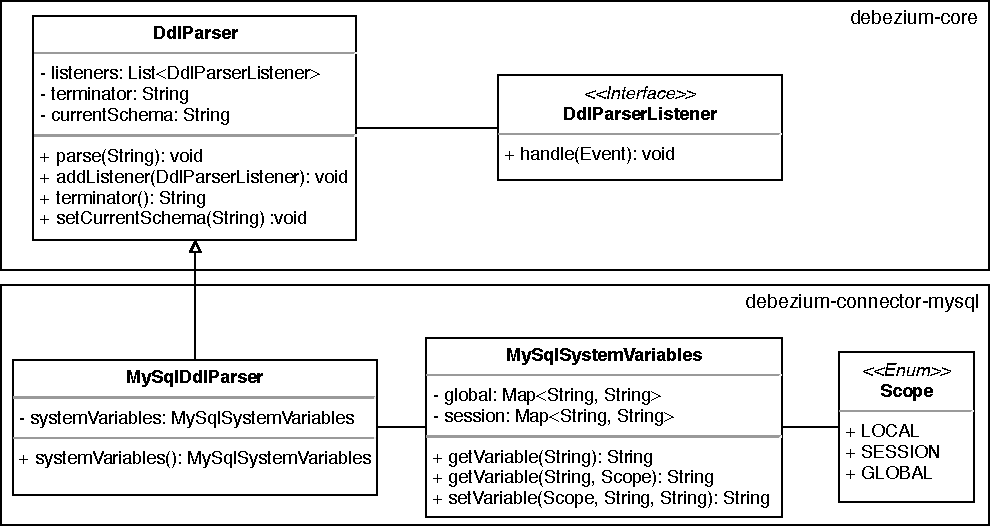
\includegraphics[width=10cm]{figures/Old_modules.pdf}
\caption{Diagram tried aktuálneho návrhu MySQL DDL parseru}
\label{fig:class_diagram_old}
\end{center}
\end{figure}

Všetky verejné metódy, ktoré obsahuje \inlinecode{DdlParser} a \inlinecode{MySqlDdlParser} predstavujú API parseru, ktoré je volané komponentou \inlinecode{MySqSchema}. 

Stávajúci návrh je viac než nedostačujúci pre možnosť rozšírenia, či už novým parserom pre MySQL databázový systém, alebo parserom pre ktorý koľvek iný DBMS. Na prvý pohľad je napríklad možné vidieť absenciu rozhrania pre \inlinecode{DdlParser}. Bližší pohľad na jedotlivé triedy z obrázku \ref{fig:class_diagram_old} nám načrtne obraz na vylepšenie tohto návrhu.

\inlinecode{DdlParser} trieda má aktuálne predstavovať základ pre všetky DDL parsre. Obsahuje implementáciu kľúčových metód, ktoré riešia: 
\begin{itemize}
\item Nastavenie DDL parseru ako napríklad, či sa majú parsovať dotazy pre náhľady tabuliek, ktoré scháma resp. databáza je aktuálne sledovaná a podobne.
\item Signalizáciu zmien nad databázou, ktoré boli počas parsovania detekované.
\item Spoločné pomocné metódy, ako napríkad metóda na vyseparovanie reťazca, ktorý je obklopený úvodzovkami a mnohé ďalšie.
\end{itemize}

Súčasťou \inlinecode{DdlParser} triedy je ale aj implementácia základnej parsovacej logiky a parsovanie konkrétnych typov reťazcov, u ktorých sa predpokladalo, že ich bude možné prepoužiť aj v rámci ďalších implementácií ddl parserov.

Trieda \inlinecode{MySqlDdlParser} predstavuje implementáciu DDL parseru. Táto trieda je už špecifická pre MySQL databázový systém, a preto nie je možné jú ďalej generalizovať. Jediným problém, ktorý u tejto implementácie nastal, je trieda \inlinecode{MySqlSystemVariables}, ktorá udržuje systémove premenné na úrovni priestoru definovaného pomocou enumu \inlinecode{Scope}. Autor túto funckionalitu implementoval ako súčasť MySQL, no správne by mala byť taktiež generalizovaná, nakoľko každý DBMS má svoje vlastné systémové premenné.

\subsection{Úprava aktuálneho designu}
Na základe nedokonalostí zistených v aktuálnom návrhu DDL parsrov, je potrebné vykonať zmeny v tomto návrhu tak, aby vyhovovali implementácii nového parseru generovaného pomocou ANTLR, ale zároveň zachvovali aktuálne riešenie a prípadnú implementáciu nových DDL parserov týmto "starým"{ }spôsobom.

Prvou zmenou v návrhu je vytvorenie rozhrania pre DDL parsre, ktoré bude definovať možnosť komunikácie pre komponenty, ktoré potrebujú parsovať DDL dotazy. Toto rozhranie bude definovať všetky verejné metódy z tried \inlinecode{DdlParser} a \inlinecode{MySqlDdlParser}. Tým sa dostávame k prvému problému, ktorým sú systemové premenné. Nakoľko nové rozhranie bude súčaťou \textit{debezium-core} modulu, je nutné generalizovať triedu \inlinecode{MySqlSystemVariables}. 

Aktuálna implemenácia triedy \inlinecode{MySqlSystemVariables} obsahuje dve \inlinecode{Map} objekty, ktoré udržiavali hodnoty systémových premenných tak, že na základe hodnoty enumu \inlinecode{Scope} bola zvolená správna mapa z ktorej sa hodnota premennej čítala. Takýto prístup v generovalizovanej verzii nie je možné použiť, nakoľko hodnoty priestoru definovaného enumom \inlinecode{Scope} sú odlišné v závislosti na DBMS. Ukladanie systémových premenných volá po riešní pomocou mapy priradenej k hodnote \inlinecode{Scope} enumu. Enum je ale špeciálny typ objektu v Jave, ktorý nedokáže dediť od iného enumu, čo prináša dilemu spojenú s tým, ako vyriešiť vlastné hodnoty \inlinecode{Scope} pre jednotlivé DBMS? 

Extendovanie enumov je väčšinou zlý nápad, no toto je jeden z prípadov kde to dáva zmysel. Možnosť ako túto situáciu vyriešiť je namiesto enumu \inlinecode{Scope} použiť rozhranie \inlinecode{Scope}. V takomto prípade majú jednotlivé implementácie možnosť vytovrenia vlastného enumu s vlastnými hodnotami kde stačí, aby tento enum implementoval rozhranie \inlinecode{Scope}. \cite{effective_java}

Nakoľko chceme prepoužiť resp. zanechať čo možno najväčiu čast stávajúcej aplikácie, bolo by vhodné vyseparovať z triedy \inlinecode{DdlParser} všetko, čo by mohola používať aj nová implmentácia parseru. Ako bolo popísané v kapitole \ref{old_design}, súčasťou implementácie \inlinecode{DdlParser} sú kľúčové metódy, ktoré nie sú závislé na štýle parsovania, a preto je vhodné ich prepoužiť aj v rámci ANTLR parseru. Vyseparujeme preto túto časť implementáciie do abstraktnej triedy, ktorá bude predstavovať najnutnejší základ pre všetky typy DDL parserov. Všetky ostatné metódy, ponecháme v \inlinecode{DdlParser}. Aby názvoslovie nebolo príliš zmätočné pozostatok triedy \inlinecode{DdlParser} predstavujúci implementáciu základnej parsovacej logiky pre ručné parsovanie nazveme \inlinecode{LegacyDdlParser} a názov \inlinecode{DdlParser} rezervujeme pre novo vytvorené rozhranie DDL parserov.

Pri každej zmene, ktorá nastane nad databázovým modelom uloženým v pamäti sa pomocou události táto zmena signalizuje poslucháčom, ktorý boli priradený DDL parseru. Myšlienka tejto funkcionality ale v stávajúcej implementácii nie je využitá. Jediným poslucháčom je \inlinecode{DdlChanges} trieda, ktorá sa tvári ako poslucháč, ale reálne tak nepracuje. Jeho reakcia na prijatú udalosť spočíva v iba v tom, že si túto událosť pridá do listu událostí, s ktorým sa následne pracuje až po ukončení práce parseru. Nakoľko neexistujú žiadny iný poslucháči, vedenie projektu sa rozhodlo túto funkcionalitu zanechat v rámci \inlinecode{LegcyDdlParser} implementácie, ale nechcelo ju mať v novej implementácii. \inlinecode{DdlChanges} trieda sa teda stane súčasťou abstraktnej implementácie parseeru a prístup k nej bude možný pomocou vystavenej metódy v rámci \inlinecode{DdlParser} rozhrania.

\begin{figure}[H]
\begin{center}
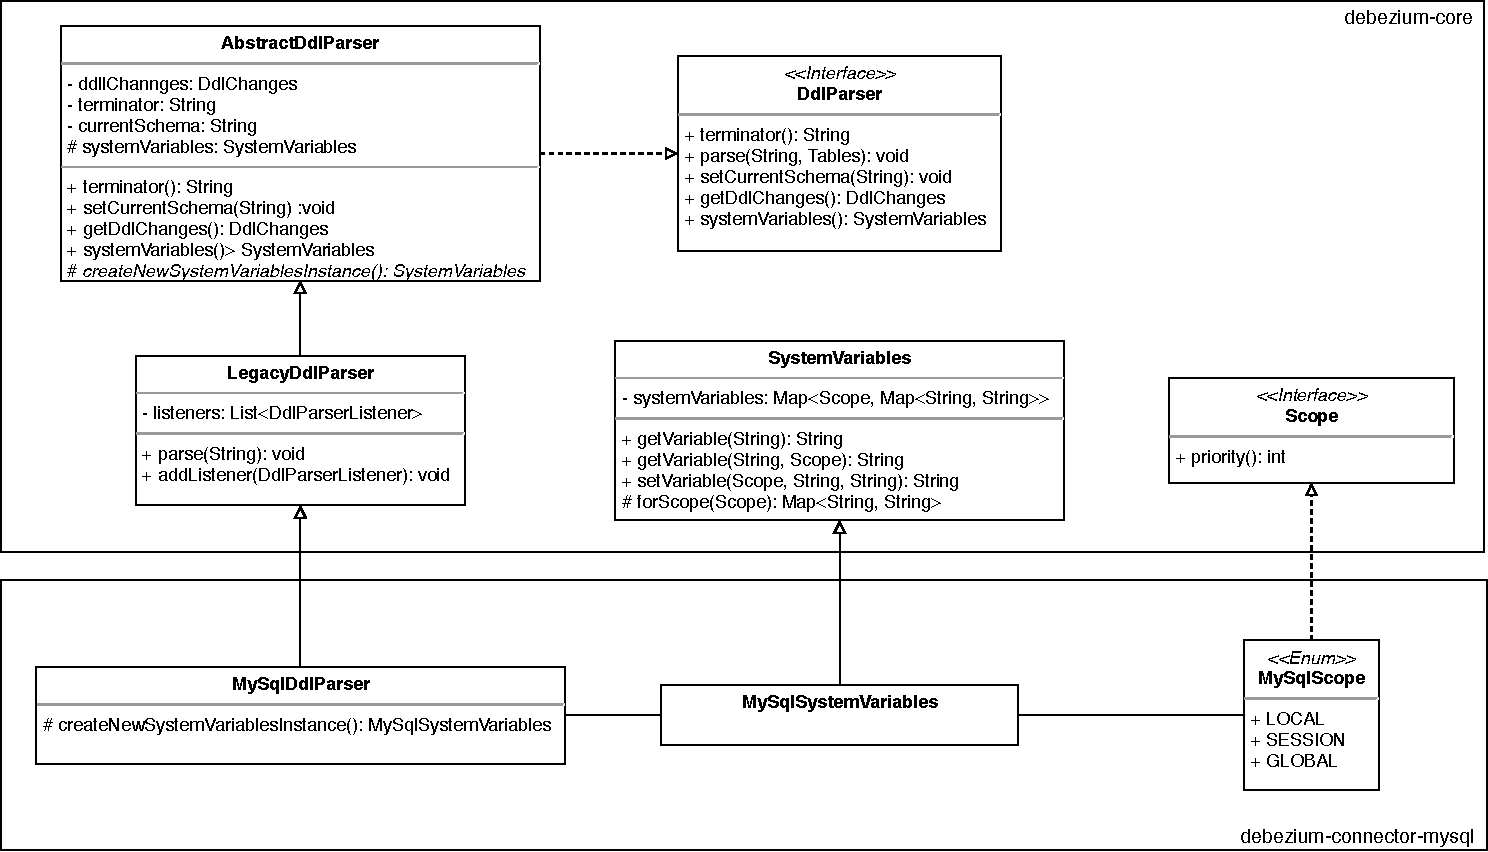
\includegraphics[width=15cm]{figures/New_design.pdf}
\caption{Upravený diagram tried MySQL DDL parseru}
\label{fig:class_diagram_new}
\end{center}
\end{figure}

\subsection{ANTLR DDL parser design}
Úpravou designu aktuálnej implementácie, ktorej výsledok je možné vidieť na obrázku \ref{fig:class_diagram_new} nám zabezpečí možnosť jednoduhšieho návrhu pre DDL parsre generované pomocou \mbox{ANTLR}. Z celého návrhu je nutné nahradiť triedy \inlinecode{LegacyDdlParser} a \inlinecode{MySqlDdlParser} za novú implementáciu. Zachovaním myšlienky na prepoužitie bude opäť návrh obsahovať triedu zo základnou implementáciou ANTLR parserov a konkrétnu implementáciu pre MySQL DBMS.

Pri návrhu je nutné počítať aj z generovaním gramatík, čo pre modul, ktorý bude definície gramatík obsahovať sposobí, že jeho build bude trvať dlhšie. Práve z dôvodu aby sa vyvojárom ušetril čas buildu pri implementovaní špecifických parserov, bude základná implementácia spolu z definíciou gramatík a vygenerovanými triedami separovaná do samostatného modulu, ktorý nazve \textbf{debezium-ddl-parser}. Samotná implementácia parseru pre MySQL, už ale bude súčasťou modulu \textit{debezium-connector-mysql}. Takýto návrh spôsobí to, že pri implementácii MySQL parseru, bude nutné buildiť modul \textit{debezium-ddl-parser} iba raz aby sa vygenerovali triedy z gramatiky a následne stačí buildiť iba modul v ktorom sa nachádza konkrétna implementácia, v rámci ktorého sa uz nič ohľadom ANTLR parseru generovať nebude.

Ako je vidieť z ukážkovej implementácie v kapitole \ref{basic_implementation}, ANTLR DDL parser sa skladá z inicializácie lexeru, parseru a priradení poslucháča, ktorý bude regovať na sparsovaný strom a vykonávať náležité akcie nad databázovým modelom, ktorý si udržuje Debezium. 
Kedže parsovací strom môže pozostávať z viacerých SQL dotazov, je potrebné počítať s tým, že v rámci jeho prechodu a snahe vykonať úpravy nad daatabázovým modelom môže nastať viacero chýb. Tieto chyby bude nutné lokálne ukladať a spracovať ich až po prejdení celého stromu. Kvôli tomu bude od konkrétnych poslúchačov vyžadované aby implementovali metódu, ktorá vráti zoznam chýb, ktoré nastali počas prechodu stromu. To sa zabezpečí použitím rozhrania \inlinecode{AntlrDdlParserListener}. 

Inicializácia lexeru a parseru je závislá na konkrétnych triedach vygenervoaných ANTLR nástrojom, ktoré majú generovaný názov podľa názvu gramatiky. To indikuje, že novú instanciu triedy musí sprostredkovávať implementácia konkrétneho parseru. Samotný postup inicializácie sa ale dá generovať a na získanie nových instancií sa môže použiť abstraktná metóda, ktorej implementácia bude súčasťou implementácia konkrétneho parseru. Ronaký poblém sa aplikuje aj na spustenie parsovania a priradenie implementácie \inlinecode{AntlrDdlParserListener}. \mbox{O inicializáciu} sa bude starať trieda \inlinecode{AntlrDdlParser}.

Výsledok tohto návrhu je možné vidieť na obrázku \ref{fig:class_diagram_antlr}.
\begin{figure}[H]
\begin{center}
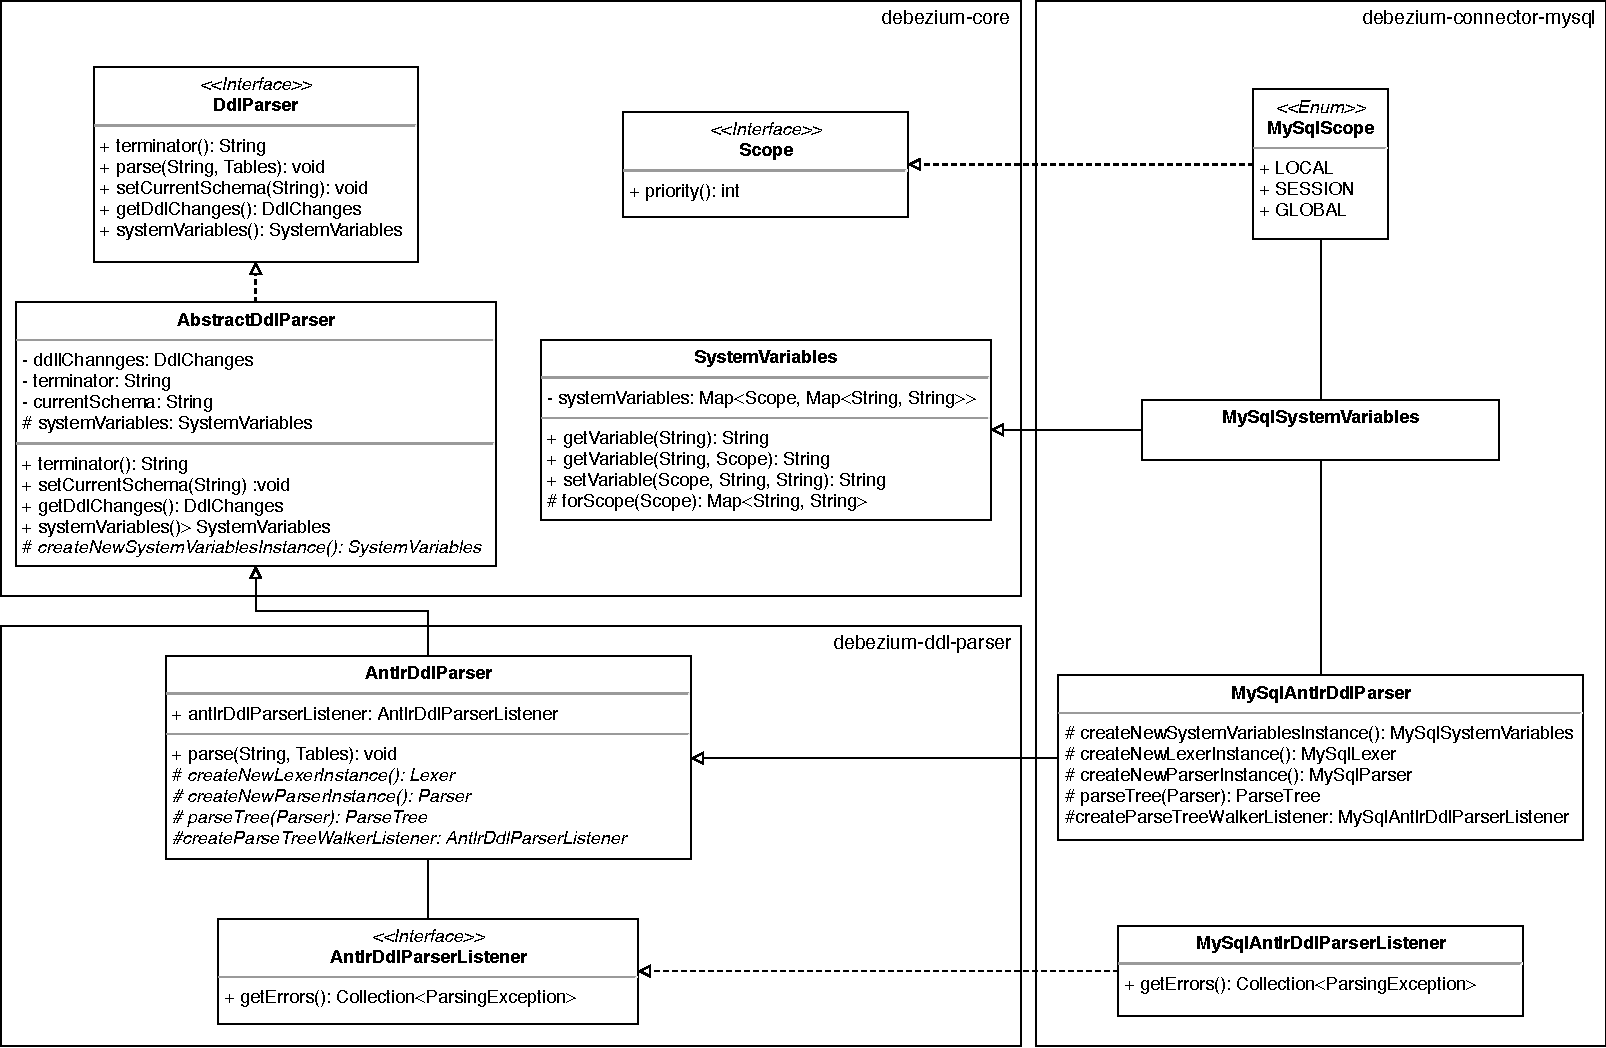
\includegraphics[width=15cm]{figures/antlr_design.pdf}
\caption{Diagram tried MySQL ANLTR DDL parseru}
\label{fig:class_diagram_antlr}
\end{center}
\end{figure}

\section{Implementácia}